\documentclass{ktuthesis}

\title{Optimizing Large Language Models for OpenAPI Completion}
\author{Bohdan Petryshyn}
\supervisor{Assoc. Prof. Mantas Lukoševičius}
\reviewer{TODO}
\authorgenitive{Studentės Studentaitės}
\addbibresource{bibliography.bib}

\usepackage[hidelinks]{hyperref}
\usepackage{lastpage}

\begin{document}
  \maketitle

  \thispagestyle{empty}
  Studentaitė, Studentė. Title of the Final Degree Project. Bachelor's  Final Degree Project / supervisor lect. Vadovas Vadovauskas; Informatics Faculty, Kaunas University of Technology.

  Study field and area (study field group): Computer Sciences, Software Systems.

  Keywords: .........(type here).

  Kaunas, \the\year. \pageref{LastPage} p.p.

  \begin{center}
    \textbf{Summary}
  \end{center}

  Lorem ipsum dolor sit amet, eam ex decore persequeris, sit at illud lobortis atomorum. Sed dolorem quaerendum ne, prompta instructior ne pri. Et mel partiendo suscipiantur, docendi abhorreant ea sit. Recteque imperdiet eum te.

  Eu eum decore inimicus consetetur, cu usu habeo corpora intellegam. Ut antiopam efficiendi deterruisset sit. Mel sint eirmod id, qui quot virtute id, dolor nemore forensibus usu id. Fugit dolore voluptatum cu vim. An vix veniam graecis insolens, sit posse iusto id. Ut vim ceteros percipit, id quo ubique recusabo, eum sint lucilius ea. In sumo inani numquam has.
  \clearpage

  \thispagestyle{empty}
  Studentaitė, Studentė. Baigiamojo projekto pavadinimas. Bakalauro studijų baigiamasis projektas / vadovas lekt. Vadovas Vadovauskas; Kauno technologijos universitetas, Informatikos fakultetas.

  Studijų kryptis ir sritis (studijų krypčių grupė): Informatikos mokslai, Programų sistemos.

  Reikšminiai žodžiai: .........(įrašykite).

  Kaunas, \the\year. \pageref{LastPage} p.p.

  \begin{center}
    \textbf{Santrauka}
  \end{center}

  Lorem ipsum dolor sit amet, eam ex decore persequeris, sit at illud lobortis atomorum. Sed dolorem quaerendum ne, prompta instructior ne pri. Et mel partiendo suscipiantur, docendi abhorreant ea sit. Recteque imperdiet eum te.

  Eu eum decore inimicus consetetur, cu usu habeo corpora intellegam. Ut antiopam efficiendi deterruisset sit. Mel sint eirmod id, qui quot virtute id, dolor nemore forensibus usu id. Fugit dolore voluptatum cu vim. An vix veniam graecis insolens, sit posse iusto id. Ut vim ceteros percipit, id quo ubique recusabo, eum sint lucilius ea. In sumo inani numquam has.

  \clearpage
  
  \tableofcontents
  \clearpage

  \listoftables
  \clearpage

  \listoffigures
  \clearpage

  \centersection{List of abbreviations and terms}

  \textbf{Abbreviations:}

  Doc. – docentas;

  Lekt. – lektorius;

  Prof. – profesorius.

  \textbf{Terms}:

  \textbf{Saityno analitika} – lorem ipsum dolor sit amet, eam ex decore persequeris, sit at illud lobortis atomorum. Sed dolorem quaerendum ne, prompta instructior ne pri. Et mel partiendo suscipiantur, docendi abhorreant ea sit. Recteque imperdiet eum te.

  \textbf{Tinklaraštis} – lorem ipsum dolor sit amet, eam ex decore persequeris, sit at illud lobortis atomorum. Sed dolorem quaerendum ne, prompta instructior ne pri. Et mel partiendo suscipiantur, docendi abhorreant ea sit. Recteque imperdiet eum te.

  Beje, darbe rekomenduojame pateikti tik svarbesnes ir mažiau žinomas santrumpas bei terminus (tarkime tokių santrumpų kaip HTML, PC, IT paaiškinti nereikia)
  \clearpage

  \centersection{Introduction}

  Supažindinama su darbo specifika, aktualumu, išdėstomi tikslai bei uždaviniai, aptariama dokumento struktūra. Šiame skyriuje apie darbą kalbama abstrakčiai, nederėtų pateikti nuorodų į kitus šaltinius (1 – 2 lapai).

  \textit{Darbo problematika ir aktualumas}

  Apibrėžiama darbo problematika ir aptariamas aktualumas. Šiame poskyryje taip pat nurodoma su darbu susijusi sritis, praktinė darbo reikšmė.

  \textit{Darbo tikslas ir uždaviniai}

  Suformuluojamas pagrindinis darbo tikslas, kuris išskaidomas į kelis uždavinius (3 – 6 uždaviniai), skirtus tikslui pasiekti. Išvados dokumento pabaigoje formuluojamos uždavinių pagrindu.
  \begin{enumerate}
    \item Pirmasis uždavinys
    \item Antrasis uždavinys
    \item Trečiasis uždavinys
  \end{enumerate}

  \textit{Darbo struktūra}

  Aptariama dokumento struktūra. Nurodoma kiek ir kokių skyrių dokumente yra ir kokia informacija juose pateikiama.

  \textit{Sistemos apimtis}

  Nors tai nėra tiesiogiai įvadinis sistemos aprašas, rekomenduojame būtent čia nurodyti jau realizuotos sistemos apimtį. Matai gali būti įvairūs: darbo valandos, kodo eilučių skaičius, komponentų, klasių, modulių kiekis, teikiamų paslaugų skaičius ir pan.

  \clearpage

  \section{Analizė}

  Su darbo problematika susijusios informacijos analizė (4 – 8 lapai). Skyriaus pavadinimas ir struktūra priklauso nuo baigiamojo darbo specializacijos ir pačios temos specifikos.

  \subsection{Techninis pasiūlymas}

  \subsubsection{Sistemos apibrėžimas}

  Nurodykite ką sistema darys. Jeigu kuriamos tik atskiros dalys, papildomai nurodykite, kurios dalys kuriamos. Galima labai neišsiplėsti, nes detaliau sistema bus aprašoma sekančiuose skyreliuose.

  Pvz.: „Maisto perdavimo protokolas (Food Transfer Protocol) – tai sistema, kuri leis žmonėms neišeinant iš namų ne tik užsisakyti, bet ir tiesiogiai parsisiųsti maisto.“

  \subsubsection{Bendras veiklos tikslas}

  Tai gali būti globalus įmonės ar abstraktus tikslas (gali būti ne vienas), kuris bus pasiektas sukūrus ir įdiegus sistemą. Aprašant nebūtina pagrįsti tikslo – nereikia aprašinėti detalių kaip tikslo ar tikslų bus siekiama. Šiame punkte taip pat aprašykite kokia nauda (tiek komercinė, tiek nekomercinė) bus gaunama įvykdžius projektą. Nauda gali būti konkretus pelnas (pvz., uždirbsite kalną pinigų), nekomercinio projekto atveju – asmeninis populiarumas (pvz., išgarsėsite savo produktu ir panaudosite tai savo ateities produktų reklamai), nauda visuomenei. Galite paminėti ir apie produkto atsipirkimą (jei tai investicinis projektas, kurio finansinė nauda planuojama tik už kelerių metų)

  Pvz.: „Maisto perdavimo protokolas leis žmonėms patenkinti maistinius poreikius jiems neišeinant iš namų“.

  \subsubsection{Sistemos pagrįstumas}

  Aprašoma pagrindinė problema, kodėl reikia kurti sistemą (kitaip tariant, iš kur kilo toks poreikis) bei sistemos aktualumas (kodėl svarbu sukurti sistemą).

  Pvz.: „Egzistuoja daug vartotojų, kurie negali arba tiesiog nenori eiti į parduotuvę ar kavinę norėdami pavalgyti. Esamos sistemos (detali analizė pateikiama sekančiame skyrelyje) nesuteikia galimybės greitai ir pigiai patenkinti maistinius poreikius, todėl šios sistemos sukūrimas iš esmės išsprendžia greito ir saugaus maisto perdavimo problemas“.

  \subsubsection{Konkurencija rinkoje}

  Panašių egzistuojančių ar šiuo metu dar tik kuriamų produktų trumpa apžvalga.

  Pvz.: „Šiuo metu egzistuoja portalai, kurie leidžia užsisakyti maistą į namus (portalo aprašymas ir funkcionalumas 1, portalo aprašymas ir jo funkcionalumas 2, <\dots>). Tačiau kol kas mano kuriamai sistemai nėra analogų“.

  Konkurentų apžvalgai iliustruoti siūloma pateikti lyginamosios analizės santrauką lentelės pavidalu (pavyzdys – \textbf{\ref{tab:comprev} lentelė}). Palyginimui svarbu pasirinkti kriterijus, pagal kuriuos įmanoma objektyviai palyginti jūsų kuriamą sistemą su konkurentais. Taip rekomenduojama, kad (pagal poreikį) kriterijai būtų įvairūs – būtų palyginamos ne tik funkcionalumas, bet ir vartotojų kiekis, kaina, operacinė sistema ar kitos ypatybės.

  \begin{table}[htbp!]
    \caption{Konkurentų apžvalga}
    \label{tab:comprev}

    \begin{tabularx}{\linewidth}{|X|>{\centering\arraybackslash}X|>{\centering\arraybackslash}X|>{\centering\arraybackslash}X|}
      \hline
      \thead[l]{Lyginimo kriterijai} & \thead{Sistema A} & \thead{Sistema B} & \thead{Sistema C}\\
      \hline
      Savybė 1 & Realizuota & Nerealizuota & Realizuota iš dalies\\
      \hline
      Savybė 2 & 1000 naudotojų\footnotemark[1] & 5000 naudotojų & 20000 naudotojų\\
      \hline
      Savybė 3 & Android & iOS & Android\\
      \hline
      Savybė 4 & + & + & -\\
      \hline
      Savybė 5 & 3.99€ & 19.99€ & Nemokama\\
      \hline
      \ldots & \ldots & \ldots & \ldots\\
      \hline
    \end{tabularx}

  \end{table}

  \footnotetext[1]{Pateikiant statistiką ar skaičius reikia nurodyti šaltinį, kurį rekomenduojama įtraukti į literatūros sąrašą}

  Po lentele taip pat rekomenduojama aprašyti palyginimo kriterijus - ką jie reiškia, kodėl jie svarbūs, kodėl buvo pasirinkti.

  \subsubsection{Prototipai ir pagalbinė informacija}

  Programą ar sistemą galima kurti ir turint tam tikrą pagrindą, t.y., modifikuojant ar ištobulinant jau esamą produktą. Jei kuriate produktą nesinaudodami
  kitu produktu kaip pagrindu, taip ir parašykite. Jei naudojatės prototipais, detaliai aprašykite kuo jūsų sprendimas geresnis už prototipą. Čia taip pat
  galite abstrakčiai parašyti, kokie informaciniai šaltiniai\footnote[2]{Šiuos informacinius šaltinius taip pat rekomenduojama įtraukti į literatūros sąrašą}
  jums labiausiai padėjo kuriant produktą (pvz., naudojotės prototipų dokumentacija ar tiesiog pasikliovėte eskperto žiniomis, klausinėjote forumuose).

  Pvz.: „Šiuo metu labiausiai paplitęs yra failų perdavimo protokolas (FTP). Vienas labiausiai išvystytų protokolų yra Bittorent, tačiau egzistuoja ir daug kur kas
  mažiau paplitusių protokolų. Tai patikimi, rinkoje įsitvirtinę protokolai. Jų didžiausias trūkumas yra tas, kad jie gali perduoti tinklu tik duomenis,
  tačiau perduoti objektus (ypač maistą) yra neįmanoma. Savo darbe daugiausiai remsiuosi FTP protokolu, nes kuriamas produktas skiriamas parduotuvei, kuri
  persiunčia nupirktą maistą klientams, \cite{litnet} t.y. veikia kaip serveris kliento-serverio architektūroje. Bittorent labiau tiktų maisto dalybai socialiniuose tinkluose“.

  \subsubsection{Ištekliai, reikalingi sistemai sukurti}

  Skyrelyje nurodykite techninių ir žmogiškųjų išteklių poreikį, kad sistema būtų sukurta.

  Pvz.: „Maisto perdavimo protokolui sukurti reikalingi 3 metai. Tiek laiko reikės aprašyti sistemos standartui ir realizuoti prototipams. Papildomai reikėtų
  10 metų, norint išpopuliarinti ir išvystyti pasaulinę protokolo infrastruktūrą. Pradinėse projekto fazėse reikės bent 10 žmonių (IT specialistų) komandos,
  tačiau projektui plečiantis turės didėti ir personalas“.

  \subsection{Galimybių analizė}

  \subsubsection{Techninės galimybės}
  Kartais sukurti galutinį produktą nepakanka finansinių, žmogiškųjų resursų ar kitų išteklių. Kliūtys gali būti tiek įmonės viduje (pvz., per smulki įmonė
  tokiam projektui realizuoti), tiek globalios (pvz., rinkoje per mažai paplitusi technika, kurią būtų galima naudoti su kuriama programine įranga, ar vartotojai
  dar nėra pasiruošę priimti produkto). Tokiu atveju reiktų detaliai aprašyti visas kliūtis, dėl kurių neįmanoma iki galo realizuoti pradinės idėjos.

  Pvz.: „Šiuo metu maisto perdavimo protokolui trūksta infrastruktūros (vamzdžių, kuriais būtų galima perduoti maistą), be to rinkoje nedaug įrenginių, kurie gali
  būti suderinami ar panaudojami bendroje protokolo veikloje. Prognozuojamas infrastruktūros ir įrenginių išplitimas – apytiksliai po 10 metų“.

  \subsubsection{Vartotojų pasiruošimo analizė}
  Jei tai produktas, kuris bus naudojamas įmonėje, tai įmonės vartotojų analizė. Jei ne – bent jau abstrakti tikslinės auditorijos (programos ar produkto vartotojų
  segmento) analizė. Šiame punkte reiktų aprašyti ar žmonės sugebės naudotis ta įranga, kokio išsilavinimo reikia norint ja naudotis.

  Pvz.: „Maisto perdavimo protokolas bus toks paprastas, kad juo galės naudotis tiek penkerių metų vaikas, tiek jo močiutė“.

  \section{Projektas}

  Aprašoma detali sistemos specifikacija (20 – 50 lapų). Apibrėžiama kuriamo produkto vizija (koncepcija). Skyriaus struktūra ir pavadinimas priklauso nuo baigiamojo
  darbo specializacijos ir pačios temos specifikos, bet turi turėti funkcinių ir nefunkcinių reikalavimų skyrius.

  \subsection{Reikalavimų specifikacija}

  \subsubsection{Komercinė specifikacija}

  Šiame skyrelyje nurodykite projekto užsakovą, projekto vykdytojus, aprašykite produkto vartotojus, detalizuokite projekto realizacijos laiko ir kainos apribojimus.
  Čia taip pat galima nurodyti verslo procesus (pvz., UML veiklos diagramomis), jei šie yra netipiniai ar reikalaujantys papildomo paaiškinimo.

  Pvz.: „Maisto perdavimu protokolas yra užsakytas Jungtinių Tautų, jį kuria 10 IT specialistų. Pagrindiniai maisto perdavimo protokolo vartotojai – Afrikos vaikai
  ir jų tėvai, tačiau sistema aktyviai naudosis ir paprasti namų vartotojai visame pasaulyje“.

  \subsubsection{Sistemos funkcijos}
  Čia būtų išvardinamos visos sistemos funkcijos (aprašomi \textbf{funkciniai reikalavimai}), pavaizduotos UML panaudojimo atvejų diagrama ar diagramomis. Po kiekvienos
  iliustracijos turi būti papildomi kiekvienos funkcijos detalūs žodiniai aprašymai. Jei norite, galite aprašyti kiekvieną panaudos atvejį išsamiai
  (PA specifikacijos lentele): atvejo pavadinimas, tikslas, aprašymas, prieš sąlyga, po sąlyga, susiję panaudojimo atvejai (\textit{include}, \textit{extend}), aktorius kt.

  \begin{figure}[htbp!]
    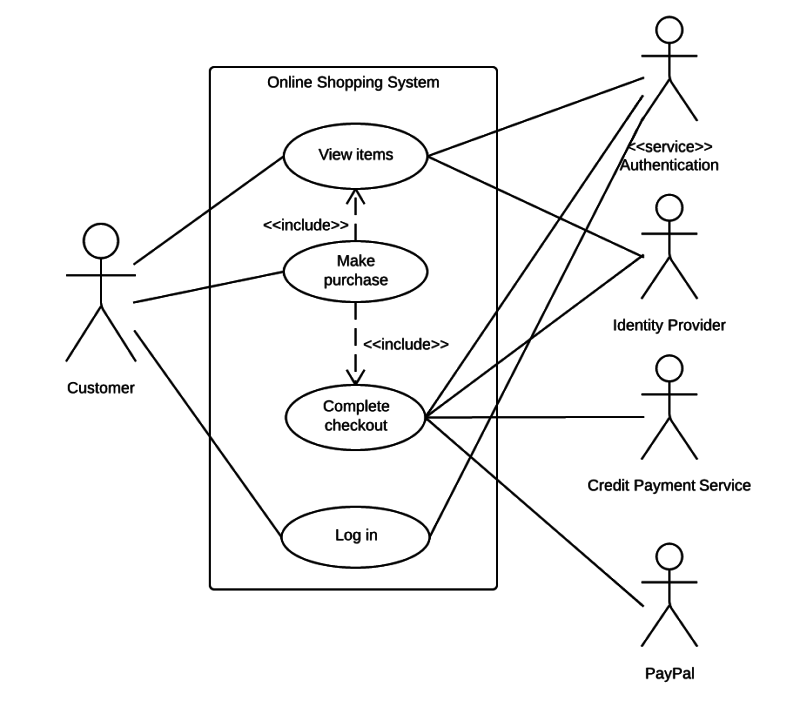
\includegraphics[width=11.22cm]{images/usecasediagram.png}
    \caption{Sistemos panaudojimo atvejų diagrama}
  \end{figure}

  \subsubsection{Vartotojo sąsajos specifikacija}

  Vartotojo sąsajos specifikacijoje turi būti nurodomi reikalavimai vartotojo sąsajos vaizdai. Čia nereikia ir negalima dėti jau egzistuojančios programos screenshot‘ų!
  Šiame etape tik nusakoma, kokia turi būti vartotojo sąsaja (rekomenduojame \textbf{Balsamiq Mockups}, \textbf{Axure RP} ir panašius įrankius), tačiau galutinis sąsajos vaizdas
  nurodomas tik vėlesniuose skyriuose. Jei pradinėje kūrimo fazėje buvo naudojami vartotojo sąsajos eskizai ar prototipai, juos reikia dėti būtent į šį skyrelį.

  \subsubsection{Realizacijai keliami reikalavimai}

  Realizacijai gali būti keliami tokie \textbf{nefunkciniai reikalavimai}: reikalavimai sistemos išvaizdai, reikalavimai panaudojamumui, reikalavimai vykdymo charakteristikoms,
  reikalavimai veikimo sąlygoms, reikalavimai sistemos priežiūrai, reikalavimai saugumui, kultūriniai-politiniai reikalavimai, teisiniai reikalavimai. Jie išvardinami
  ir aprašomi šiame skyrelyje. Pavyzdžiui:
  \begin{enumerate}
    \item Maisto perdavimo protokolas privalo būti saugus (neautentifikuoti kaimynai negali sužinoti, kokį maistą siunčiasi vartotojas)
    \item Maistas suskaidytas paketais, turi pasiekti vartotoją nepagedęs
    \item Maisto perdavimo protokolas turėtų palaikyti lietuviškos virtuvės produktus
  \end{enumerate}

  Šiame punkte gali būti išvardinti (jeigu nustatyti) tokio tipo apribojimai: apribojimai sprendimui, diegimo aplinka, bendradarbiaujančios sistemos, komerciniai
  specializuoti programų paketai, numatoma darbo vietos aplinka, sistemos kūrimo terminai, sistemos kūrimo biudžetas. Jei reikalinga specifinė duomenų kontrolė
  (kokia informacija turi būti tikrinama įvedimo ar sistemos veikimo metu), ji taip pat aprašoma šiame skyrelyje.

  \subsubsection{Techninė specifikacija}

  Skyrelyje aprašykite techninę ir papildomą programinę įrangą, reikalingą sistemai. Nurodykite minimalius įrangos parametrus. Šis skyrelis, priklausomai nuo
  situacijos, gali būti formuluojamas kaip sąrašas, ką užsakovams reikės turėti, jeigu norės naudotis sistema, arba kokios aplinkos reikalauja užsakovas.

  Pvz.: „Maisto perdavimo protokolui realizuoti būtinas interneto ryšys, 1 kilolitro maisto ir gėrimų perdavimo linija, specializuotas šaldytuvas, namų kompiuteris“.

  \subsection{Projektavimo metodai}

  \subsubsection{Projektavimo valdymas ir eiga}

  Šiame punkte nurodykite, kokį programinės įrangos kūrimo modelį (ar modelius) naudojote kurdami savo sistemą. Tai gali būti krioklio, iteracinis ar kitas modelis.
  Galite nurodyti kaip suskirstėte darbus ir kokiu eiliškumu juos atlikote.

  \subsubsection{Projektavimo technologija}

  Šiame punkte nurodykite, kokią naudojote projektavimo technologiją, standartus ir programinius įrankius projekto kūrimui. Aprašykite kokia ar kokiomis notacijomis
  (formaliais tekstiniais ir grafiniais žymėjimo / aprašymo standartais) naudojotės kurdami sistemos projektą.

  \subsubsection{Programavimo kalbos, derinimo, automatizavimo priemonės, operacinės sistemos}

  Šiame punkte, tiesiog, aprašykite, kokią programinę įrangą naudojote kurdami savo baigiamąjį darbą. Tiesa, rašyti kokią programinę įrangą naudojote šiai ataskaitai
  sukurti – nebūtina.

  \subsection{Sistemos projektas}

  Sistemos projektas – tai jūsų sistemos veikimo aprašymas. Tai dažniausiai nagrinėjama dokumento vieta (be išvadų) darbo peržiūros ir gynimo metu.

  \subsubsection{Statinis sistemos vaizdas}

  Šiame punkte reikėtų detalizuoti sistemos struktūrą. Priklausomai nuo projekto tipo (rekomenduojame pasikonsultuoti su vadovu) turėtumėte aprašyti
  savo sistemą panaudodami UML diagramas:
  \begin{itemize}[label={--}]
    \item Išdėstymo (angl. \textit{UML deployment diagram}) – nepakeičiama tuo atveju, jei sistema naudoja išorinius servisus ar yra paskirstyta
    per keletą įrenginių. Geriausia pradėti nuo šios diagramos, nes ji greičiausiai supažindina su bendra sistemos sudėtimi.
    \item Komponentų (angl. \textit{UML component diagram}) – geriausiai tinka tuomet, kai naudojamas komponentinis sistemos kūrimo būdas ir sistema
    susideda iš komponentų teikiančių programavimo sąsają (API).
    \item Paketų (angl. \textit{UML package diagram}) - labai naudinga tuomet, jei sistema sugrupuota paketais.
    \item Klasių (angl. \textit{UML class diagram}) - geriausiai tinka atvaizduoti sistemos struktūros detales. Jei projekte klasių naudojama daug,
    rekomenduojama detalizuoti tik esmines klases, o likusią struktūrą pateikti paketų diagrama.
    \item Aprašant statinį sistemos vaizdą taip pat turėtų būti pateikta ir duomenų bazės schema. Šiam tikslui gali būti naudojama esybių ryšių diagrama arba (geriausia)
    UML klasių diagrama. Jei naudojama ne reliacinė duomenų bazė, tuomet naudoti tokį duomenų bazės specifikavimo būdą, kurį siūlo kūrėjai arba bendruomenė.
  \end{itemize}

  \subsubsection{Dinaminis sistemos vaizdas}

  Dinaminiame sistemos vaizde parodoma kaip sistema veikia naudojama. Šiame
  punkte pagal poreikį galima pavaizduoti sistemos veiksmus UML veiklos, sekų
  ir/arba būsenų diagramomis. Galite pasirinkti vieną iš jų, galite naudoti ir
  kelias (priklausomai nuo sistemos specifikos).

  \section{Testavimas}

  Aprašoma su sukurtos įrangos testavimu susijusi informacija (8 – 12 lapai). Skyriaus struktūra ir pavadinimas priklauso nuo baigiamojo darbo
  specializacijos ir pačios temos specifikos.

  Nurodomas įrangos testavimo planas, testavimo duomenų rinkiniai ir gauti rezultatai. Nurodoma sistemos specifikacija ir sąlygos, prie kurių
  buvo atliekamas testavimas.

  \subsection{Testavimo planas}

  Testavimo planas – tai jūsų pasirinkta testų atlikimo tvarka. Galimas testavimo planas: komponentų testavimas, po kurio seka integracinis
  testavimas, o vėliau būna sąsajos testavimas.

  \subsection{Testavimo kriterijai}

  Šiame punkte aprašykite kriterijus, kurie jums buvo svarbūs testavimo metu. Tai gali būti ne tik informacijos ar skaičiavimų korektiškumas,
  bet ir kodo pertekliškumo analizė, informacijos perdavimo laikas, sistemos atitikimas funkciniams ir nefunkciniams reikalavimams.

  \subsection{Komponentų testavimas}

  Šiame punkte reiktų aprašyti kokiais metodais testavote smulkias programos dalis (žr. wiki \textit{unit testing}). Komponentų testavimas privalo būti
  atliekamas naudojant automatines testavimo priemones.

  \subsection{Integracinis testavimas}

  Jei kurdami sistemą atlikote integracinį testavimą, jį aprašykite šiame skyrelyje. Integracinis testavimas privalo būti atliekamas naudojant automatines testavimo priemones.

  \subsection{Vartotojo sąsajos testavimas}

  Šiame punkte reiktų aprašyti kokiais metodais testavote vartotojo sąsają. Dažniausiai pasitaikantis metodas – „rankinis“, t.y. kai sąsaja testuojama
  vartotojui (testuotojui) bandant atsitiktinai ar pagal scenarijų spaudyti mygtukus, įvedinėti tekstą į laukus ir kt. Kur kas geresnis variantas tuomet,
  kai testuojama automatiškai – pavyzdžiui, sukuriama programa ar testavimo tvarkyklė, kuris spaudymo ar įvedimo veiksmus atlieka be vartotojo įsikišimo.
  Panaudotas automatinis testavimas, dažniausiai, papildomai (teigiamai) įvertinamas baigiamojo darbo gynimo metu. Pasinaudokite automatizavimo priemonėmis,
  tokiomis kaip \textbf{Selenium IDE}.

  \section{Dokumentacija naudotojui}

  Dokumento dalis, skirta naudotojui, kur aprašomas visas naudotojui aktualus programinės (aparatūrinės) įrangos funkcionalumas (4 – 10 lapų).

  Dokumentacija naudotojui – tai instrukcija kaip naudotis sistema. Dokumentacijoje turi būti aiškiai aprašyti naudojimosi sistema ypatumai, pradedant
  diegimu ir baigiant įprastinėmis funkcijomis. Rašydami dokumentaciją atsižvelkite į naudojamą terminologiją. Pavyzdžiui, jei sistemą instaliuos administratorius,
  o naudos paprasti vartotojai, pastarųjų stenkitės neapkrauti sudėtingesnėmis sąvokomis.

  \subsection{Apibendrintas sistemos galimybių aprašymas}

  Sistemos galimybės nuo reikalavimuose aprašyto funkcionalumo skiriasi tuo, kad ne visiems vartotojams būtina žinoti technines projekto detales.
  Pavyzdžiui, internetinio portalo vartotojui svarbu žinoti kokios naudingos funkcijos yra portale (pvz., paieška, naujienlaiškio prenumerata ir kt.),
  tačiau ne visos funkcijos įprastam vartotojui yra aktualios (pvz., reklamos skydelių palaikymas, SSL protokolas vartotojų autentifikacijai ir t.t.).

  Ši pastraipa skirta nuorodoms į literatūros sąrašą: \cite{litnet}, \cite{ontologies}, \cite{valstybestarnyba}, \cite{spaudosdraudimas}, \cite{krastoapsauga}, \cite{citationguide}, \cite{velomobilis}.

  \subsection{Vartotojo vadovas}

  Vartotojo vadovas yra neformalus įvadas į sistemą, aprašantis jos „normalų“ vartojimą. Kitaip tariant, vartotojui draugiška instrukcija su daug
  iliustracijų ir paaiškinimų. Neišvengiamai pradedantieji, nepriklausomai nuo patirties, daro klaidas. Lengvai randama informacija, kaip nuo šių
  klaidų grįžti prie naudingo darbo ir atstatyti galimus klaidų padarinius, turi būti sudėtinė šio dokumento dalis.

  \subsection{Diegimo vadovas}

  Sistemos diegimo dokumentas yra skiriamas sistemos administratoriams (dažniausiai tai kompiuterius prižiūrintis personalas, tačiau šie žmonės
  nebūtinai būna ir sistemos naudotojai). Jame turi būti nurodytos diegimo konkrečioje aplinkoje detalės, turi būti supažindinama su sistemą
  sudarančiais failais, minimalia reikalingos techninės įrangos konfigūracija.

  \subsection{Administravimo vadovas}

  Sistemos administratoriaus vadove turi būti aprašyti pranešimai, kaip sistema bendrauja su kitomis sistemomis ir kaip reaguoti į šiuos pranešimus.
  Būtų gerai nurodyti, kaip reaguoti į sistemos klaidas (sisteminių pranešimų paaiškinimai). Jei sistema apima ir techninę įrangą, jame turi būti
  aprašyti operatoriaus veiksmai palaikant šią techninę įrangą (pvz., kaip prijungti naujus periferinius įrenginius ir t.t.).

  \newpage

  \centersection{Conclusions}

  Bene svarbiausia viso darbo dalis – išvados. Išvados nenurodo, kas buvo padaryta darbe, bet pabrėžia atrastus dėsningumus, pastebėtas technologijų
  ar rinkos spragas, esminius įrangos privalumus. Išvados gali būti formuluojamos tik darbo metu sukurtos įrangos, technologijos, metodo ar susistemintos
  informacijos pagrindu (pvz., negalima cituoti šaltinių, vadovautis kitų autorių atrastais dėsningumais).
  Išvados numeruojamos, jų turėtų būti maždaug 4-9 (pvz., kiekvienam kūrimo etapui – reikalavimų analizei, projektavimui, realizacijai, testavimui, diegimui).
  Įprastai kiekviena išvada turėtų būti sudaryta iš atlikto veiksmo aprašymo ir gautų rezultatų. Išvadas galima gauti:
  \begin{itemize}[label={--}]
    \item Atlikus konkurentų analizę, kuomet būna išsiaiškinama esminiai konkurentų sistemų pranašumai ir trūkumai (pvz., „Buvo išanalizuotos analogiškos
    (konkrečiai nurodant kokios) sistemos, kurios pasižymėjo tokiais ir tokiais privalumais (apibendrintai), tačiau dėl tokių ar anokių trūkumų buvo
    nuspręsta kurti naują sistemą...“).
    \item Atlikus technologijų analizę, kuomet būna pagrindžiamas konkrečių programavimo kalbų, karkasų ar kitų technologijų pasirinkimas
    (pvz., „Išanalizavus x, y ir z technologijas buvo pasirinkta technologija z. Tai padėjo lengviau suprojektuoti, o vėliau ir realizuoti įrankio serverio
    pusės dalį, palaikyti vientisą programos kodo struktūrą...“).
    \item Atlikus testavimą, kuomet būna nurodoma kokį kodo padengimą pavyko pasiekti, kokias klaidas pavyko aptikti panaudojus pasirinktus testavimo metodus.
    \item Susidūrus su tam tikromis specifinėmis problemomis, kurioms išspręsti buvo panaudotas jūsų sugalvotas metodas („Kūrimo metu buvo susidurta su tokiomis
    ar anokiomis problemomis, kurios buvo sprendžiamos taip arba anaip...“). Galima įdėti ir išvadą apie nepasiteisinusius, tačiau jūsų išbandytus sprendimus
    (siekiant, kad kiti „neliptų ant to paties grėblio“). Jūsų parinkti problemų sprendimo būdai yra svarbios išvados, parodančios jūsų kompetenciją ir įsigilinimą į darbą.
    \item Realizavus pačią programą ar sistemą, kuri (greičiausiai) pakeitė ar pagerino iki tol vykusius verslo procesus (tai susiję su skyreliais „Bendras veiklos tikslas“
     ir „Sistemos pagrindimas“) ar (jei tai buvo mokslinio pobūdžio darbas) tiesiog iki tol buvusius algoritmo / sprendimo rezultatus.
  \end{itemize}

  Šiame skyrelyje taip pat būtina pridėti ir papildomas išvadas-rezultatus apie tai:
  \begin{itemize}[label={--}]
    \item Kokia yra sistemos esama būklė. Verta paminėti, jei sistema yra praktiškai naudojama įmonėje ar (programėlės kūrimo atveju) programėlė yra įkelta
    į Google Play ar AppStore parduotuves.
    \item Kas planuojama atlikti tobulinant sistemą ateityje. KAdangi baigiamajam darbui sukurti yra skiriamas ribotas laikas, galbūt verta paminėti tas savybes,
    kurių dėl laiko apribojimų tiesiog nespėjote, bet planuojate įgyvendinti.
  \end{itemize}

  \clearpage
  \addcontentsline{toc}{section}{List of references}
  \printbibliography[title={\hfil\fontsize{12}{15}\selectfont{List of references}}]

  \newpage
  \centersection{Appendices}

  \appendix
  \renewcommand{\thesection}{\arabic{section}}

  \section{Priedo pavadinimas}

  \section{Antras priedas}

\end{document}
